\chapter{Contexte general du projet :}
\section{Presentation du centre :}
Le Code 212 est un centre de formation et de certification dans les metiers du digital, lance dans le cadre du Plan d'Acceleration de la Croissance et de la Transformation de l'economie (PACTE) ESRI-2030 au Maroc. Ce programme vise à repondre aux enjeux actuels et futurs lies à l'emergence des technologies numeriques en offrant des filières specifiques et des formations certifiantes. L'objectif est de renforcer les competences et les qualifications dans le secteur numerique, contribuant ainsi à l'atteinte des objectifs de developpement du pays, notamment celui de faire passer la part du secteur numerique à 5% du PIB d'ici 2035.

Le principal objectif du Centre Code 212 est de former une nouvelle generation de professionnels qualifies dans le domaine du numerique afin de repondre aux besoins croissants du marche de l'emploi dans ce secteur en plein essor. En offrant des formations specialisees et des certifications reconnues, le centre vise à fournir aux apprenants les competences et les connaissances necessaires pour reussir dans des domaines tels que le developpement web, la cybersecurite, l'analyse de donnees, le marketing digital et bien d'autres. En outre, le centre s'engage à promouvoir l'innovation et l'entrepreneuriat en encourageant les initiatives creatives et en offrant un environnement propice à l'emergence de projets novateurs dans le domaine du digital.

\subsection{Fiche du centre Code 212}

\begin{tabularx}{\textwidth}{|l|X|}
\hline
\textbf{Nom du Centre} & Code 212 \\
\hline
\textbf{Domaine d'Activite} & Formation et certification dans les metiers du digital \\
\hline
\textbf{Programme} & Plan d'Acceleration de la Croissance et de la Transformation de l'economie (PACTE) ESRI-2030 \\
\hline
\textbf{Localisation} & Agadir Maroc \\
\hline
\textbf{Objectif} & Renforcer les competences et les qualifications dans le secteur numerique \\
\hline
\textbf{Domaines de Formation} & 
\begin{tabular}{@{}l@{}}
- Developpement web \\
- Cybersecurite \\
- Analyse de donnees \\
- Marketing digital \\
- et bien d'autres
\end{tabular} \\
\hline
\textbf{Engagement} & 
\begin{tabular}{@{}l@{}}
- Promouvoir l'innovation \\
- Encourager l'entrepreneuriat \\
- Offrir un environnement propice aux projets novateurs
\end{tabular} \\
\hline
\end{tabularx}


\subsection{Centre Code212}
\begin{figure}[H]
\centering
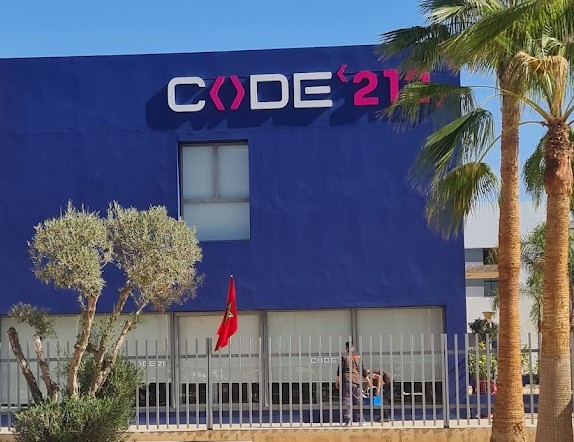
\includegraphics[height=10cm , width=\textwidth]{assets/images/code.jpg}
\caption{Centre Code 212 Agadir}
\label{fig:imagecentre}
\end{figure}

\begin{figure}[H]
\centering
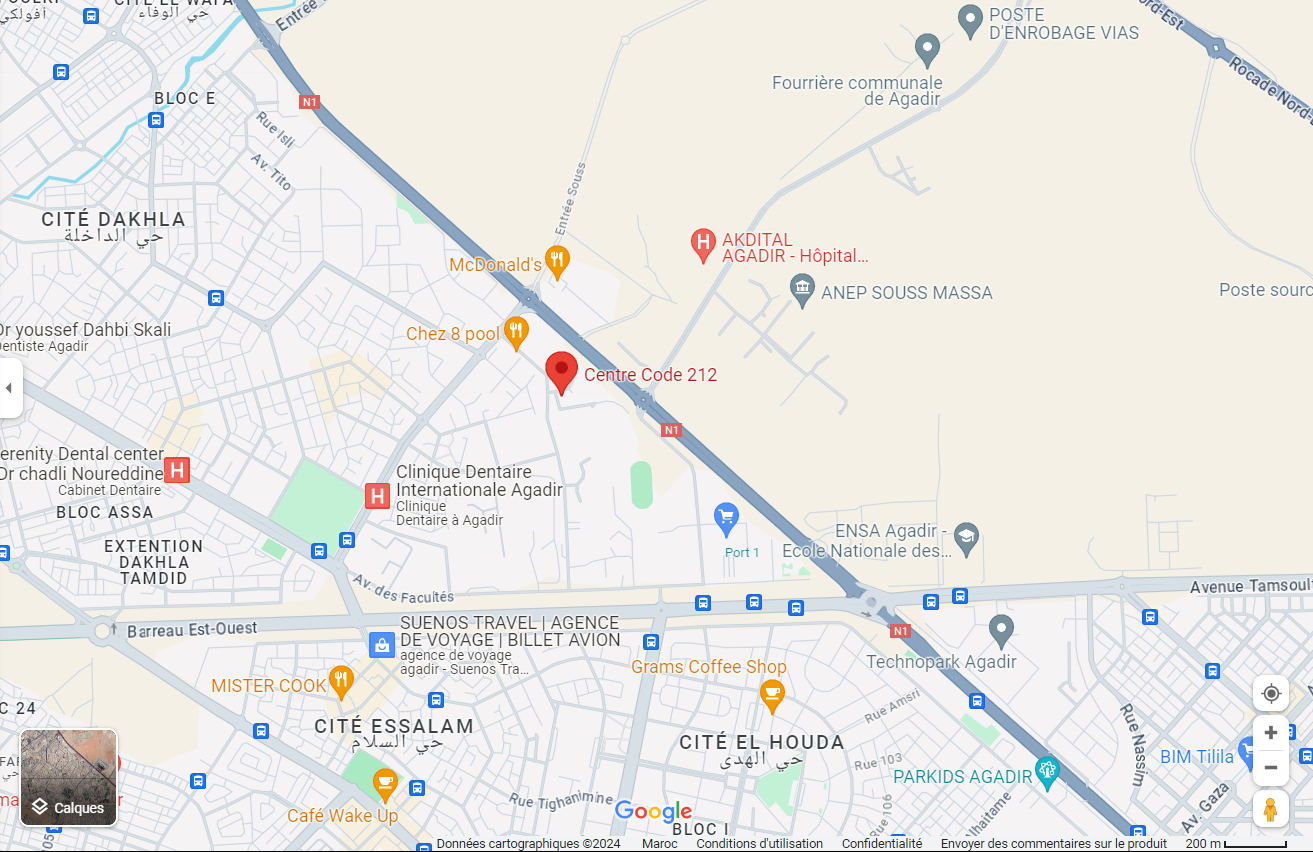
\includegraphics[height=10cm , width=\textwidth]{assets/images/maps.png}
\caption{Localisation du centre}
\label{fig:localisationcentre}
\end{figure}

\subsection{Domaines d'activites et expertise :}

Le centre Code 212 d'Agadir developpe son expertise autour de plusieurs axes strategiques, visant à repondre aux exigences du marche numerique moderne et aux besoins de transformation digitale du Maroc.

\subsubsection{Education et Pedagogie innovante :}

\paragraph{Methodologie d'apprentissage :}
L'education au sein du centre Code 212 repose sur une approche pedagogique revolutionnaire qui rompt avec les methodes traditionnelles d'enseignement. Cette methode, connue sous le nom de \textbf{peer-to-peer learning}, place l'apprenant au centre du processus educatif et favorise :

\begin{itemize}
    \item \textbf{Apprentissage collaboratif} : Les etudiants travaillent en equipes pour resoudre des projets concrets, simulant ainsi l'environnement professionnel reel
    \item \textbf{Autonomie pedagogique} : Absence de cours magistraux traditionnels, encourageant l'auto-apprentissage et la recherche personnelle
    \item \textbf{Mentorat mutuel} : Les etudiants avances accompagnent les debutants, creant une dynamique d'entraide et de partage de connaissances
    \item \textbf{Evaluation par les pairs} : Systeme d'evaluation base sur la correction mutuelle des projets
\end{itemize}

\paragraph{Infrastructure technologique :}
Le centre dispose d'equipements de pointe incluant :
\begin{itemize}
    \item Laboratoires informatiques equipes de stations de travail haute performance
    \item Plateforme d'apprentissage en ligne personnalisee
    \item Environnements de developpement integres (IDE) professionnels
    \item Acces aux technologies cloud et aux outils de developpement modernes
\end{itemize}

\subsubsection{Renforcement des competences et employabilite :}

\paragraph{Programmes de formation specialises :}
Code 212 Agadir propose un curriculum adapte aux exigences du marche du travail numerique, structuré autour de plusieurs piliers :

\begin{enumerate}
    \item \textbf{Socle technique fondamental :}
    \begin{itemize}
        \item Algorithmique et structures de donnees
        \item Programmation orientee objet
        \item Bases de donnees et gestion de l'information
        \item Architectures logicielles et design patterns
    \end{itemize}
    
    \item \textbf{Technologies emergentes :}
    \begin{itemize}
        \item Intelligence artificielle et machine learning
        \item Developpement web full-stack (Frontend/Backend)
        \item Applications mobiles natives et cross-platform
        \item Cloud computing et DevOps
        \item Cybersecurite et protection des donnees
    \end{itemize}
    
    \item \textbf{Competences transversales :}
    \begin{itemize}
        \item Gestion de projets agiles (Scrum, Kanban)
        \item Travail en equipe et communication
        \item Entrepreneuriat et innovation
        \item Veille technologique et apprentissage continu
    \end{itemize}
\end{enumerate}

\paragraph{Partenariats et insertion professionnelle :}
Le centre maintient des relations etroites avec l'ecosysteme economique local et national :
\begin{itemize}
    \item \textbf{Partenariats entreprises} : Collaboration avec des startups et des multinationales pour des projets reels
    \item \textbf{Stages professionnels} : Programme de stages obligatoires en entreprise
    \item \textbf{Job dating} : Organisation regulière d'evenements de recrutement
    \item \textbf{Incubation} : Accompagnement des projets entrepreneuriaux des etudiants
\end{itemize}

\paragraph{Suivi et accompagnement :}
\begin{itemize}
    \item Coaching personnalise pour chaque etudiant
    \item Suivi post-formation pendant 12 mois
    \item Reseau alumni actif
    \item Formation continue et certification professionnelle
\end{itemize}

\section{Presentation du projet :}

\subsection{Problematique et presentation du projet}

Avec l'essor des medias numeriques et des plateformes d'actualites en ligne au Maroc, l'analyse des sentiments exprimés par les utilisateurs dans les commentaires devient cruciale pour comprendre l'opinion publique. Hespress, l'un des sites d'actualites les plus populaires au Maroc, reçoit quotidiennement des milliers de commentaires sur ses articles, representant une source riche d'informations sur les sentiments et opinions des citoyens marocains.

Face à ce volume important de donnees textuelles, il devient necessaire de developper un systeme automatise capable d'analyser et de classer les sentiments exprimés dans ces commentaires de manière efficace et precise.

\subsection{Contexte de l'analyse de sentiments}

Le contexte actuel des medias numeriques est marque par une participation active des citoyens qui expriment leurs opinions à travers les commentaires. Cette interaction massive genere une quantite considerable de donnees non structurees qui necessitent des outils d'analyse avancés pour en extraire des informations pertinentes.

\subsection{Besoin d'une analyse automatisee}

À l'ere du big data, où les volumes de donnees textuelles croissent exponentiellement, les organisations et les chercheurs ont besoin d'outils capables d'analyser automatiquement les sentiments exprimés dans les textes. Un systeme d'analyse de sentiments s'avere indispensable pour traiter efficacement ces grandes quantites de donnees et en extraire des insights significatifs.

\section{Solution Proposee}

L'application d'analyse de sentiments represente une solution innovative pour traiter et analyser les commentaires d'Hespress. Capable de collecter, traiter et classer automatiquement les sentiments exprimés, elle offre une analyse en temps reel des opinions publiques.

\subsection{Architecture de l'application}

L'application sera developpee avec une architecture moderne et scalable utilisant les technologies suivantes :

\begin{itemize}
    \item \textbf{Frontend} : Next.js pour une interface utilisateur moderne et reactive
    \item \textbf{Backend} : FastAPI pour une API rapide et performante
    \item \textbf{Authentification} : Keycloak pour la gestion securisee des utilisateurs
    \item \textbf{Web Scraping} : Selenium pour la collecte automatisee des commentaires
    \item \textbf{Analyse de sentiments} : Modele cardiffnlp/twitter-xlm-roberta-base-sentiment pour la classification des textes
    \item \textbf{API Gateway} : Spring pour la gestion et la securisation des APIs
\end{itemize}

\subsection{Methodes d'analyse de sentiments}

Pour l'analyse de sentiments, nous utilisons le modele pre-entraine \textbf{cardiffnlp/twitter-xlm-roberta-base-sentiment}, specifiquement optimise pour l'analyse de sentiments sur des textes courts et informels, similaires aux commentaires sur les reseaux sociaux.

\subsubsection{Le modele XLM-RoBERTa}

XLM-RoBERTa est un modele de langage multilingue base sur l'architecture Transformer, pre-entraine sur des donnees textuelles dans plusieurs langues, incluant l'arabe et le français, ce qui le rend particulièrement adapte au contexte marocain.

\paragraph{Avantages du modele choisi :}
\begin{itemize}
    \item \textbf{Support multilingue} : Capable de traiter les textes en arabe, français et darija marocaine
    \item \textbf{Optimisation pour les reseaux sociaux} : Entraine specifiquement sur des donnees de Twitter
    \item \textbf{Precision elevee} : Performance demontree sur les taches de classification de sentiments
    \item \textbf{Facilite d'integration} : Disponible via la librairie Transformers de Hugging Face
\end{itemize}

\paragraph{Processus d'analyse :}
\begin{itemize}
    \item Collecte automatisee des commentaires via Selenium
    \item Preprocessing et nettoyage des textes
    \item Tokenisation et preparation des donnees pour le modele
    \item Classification des sentiments (positif, negatif, neutre)
    \item Stockage et visualisation des resultats
\end{itemize}

\section{Tableau des fonctionnalites}

Nous presentons ici un tableau decrivant les fonctionnalites offertes par l'application d'analyse de sentiments et leur impact sur l'analyse des donnees.

\begin{table}[H]
\centering
\begin{tabularx}{\textwidth}{|l|X|}
\hline
\textbf{Fonctionnalite} & \textbf{Description et Impact} \\
\hline
Collecte automatisee des commentaires & 
L'application collecte automatiquement les commentaires d'Hespress en temps reel, permettant une analyse continue et actualisee des sentiments exprimés. \\
\hline
Classification des sentiments & 
Analyse et classification automatique des sentiments (positif, negatif, neutre) avec une precision elevee grace au modele XLM-RoBERTa. \\
\hline
Tableau de bord analytique & 
Interface intuitive pour visualiser les resultats d'analyse avec des graphiques et des statistiques en temps reel. \\
\hline
Gestion des utilisateurs & 
Systeme d'authentification securise avec Keycloak permettant la gestion des droits d'accès et des profils utilisateurs. \\
\hline
API RESTful & 
Interface de programmation robuste pour l'integration avec d'autres systemes et l'accès aux donnees d'analyse. \\
\hline
Historique et tendances & 
Suivi des tendances de sentiments dans le temps avec possibilite d'analyse historique et de generation de rapports. \\
\hline
\end{tabularx}
\caption{Recapitulatif des fonctionnalites de l'application d'analyse de sentiments}
\label{tab:fonctionnalites}
\end{table}

\section{Conduite du Projet}

La conduite efficace du projet de developpement de l'application d'analyse de sentiments est essentielle pour repondre aux exigences specifiques d'analyse des commentaires d'Hespress. Cette section explore en detail les processus de conception, de planification et de developpement qui sous-tendent la creation de l'application.

\subsection{Conception}

La phase de conception constitue l'etape fondatrice du projet, où l'equipe definit les objectifs de l'application, identifie les fonctionnalites cles et elabore l'architecture generale du systeme d'analyse de sentiments. Cette phase necessite une comprehension precise des besoins d'analyse et des caracteristiques specifiques des commentaires d'Hespress.

À ce stade, des etudes de faisabilite technique, des analyses de performance des modeles de NLP et des sessions de definition des exigences avec les parties prenantes sont utilisees pour rassembler les specifications et pour esquisser les premiers prototypes de l'interface utilisateur. Les scenarios d'utilisation et les workflows d'analyse sont methodiquement elabores pour garantir que l'application est à la fois performante et techniquement viable.

\subsection{Planification des Taches}

Une planification detaillee accompagne une conception reussie ; elle s'attaque à la complexite du processus de developpement en decomposant le projet en modules gererables. L'equipe du projet etablit un calendrier de realisation, determinant les dependances entre les composants et en allouant les ressources necessaires.

La methodologie Agile est adoptee, permettant une flexibilite et une reactivite accrues face aux changements de requirements ou aux retours des utilisateurs. La creation de sprints, la priorisation des backlogs et les revues regulières de sprint assurent que le projet reste sur la bonne voie et adapte aux exigences changeantes tout au long de son cycle de vie.

\subsection{Developpement et Integrations}

Durant la phase de developpement, l'equipe met en œuvre la conception de l'application en codant les differentes composantes logicielles. Les developpeurs integrent les technologies choisies : Next.js pour le frontend, FastAPI pour le backend, Keycloak pour l'authentification, et le modele de sentiment analysis.

La construction de l'infrastructure technique, comprenant les serveurs, les bases de donnees et l'integration avec les APIs, est rigoureusement testee pour garantir son bon fonctionnement. Une serie exhaustive de tests—tests unitaires, tests d'integration et tests de performance—est realisee pour s'assurer que le systeme est robuste, evolutif et pret pour le deploiement.

\section{Methodologie Scrum et ses roles}

Scrum est une methodologie agile utilisee principalement dans le developpement de logiciels pour gerer des projets complexes et assurer une livraison continue de produits de haute qualite. Elle repose sur des cycles de developpement iteratifs et incrementaux appeles "sprints", qui durent generalement de deux à quatre semaines. Scrum encourage la collaboration, la flexibilite et l'amelioration continue à travers des revues regulières et des retrospectives.

\subsection{Les roles dans Scrum}

\begin{itemize}
    \item \textbf{Product Owner (PO)} : Le Product Owner est responsable de maximiser la valeur du produit resultant du travail de l'equipe de developpement. Il gère le backlog produit, un document evolutif contenant les exigences et les fonctionnalites du produit, en le priorisant selon la valeur ajoutee pour le client et les parties prenantes.
    
    \item \textbf{Scrum Master} : Le Scrum Master est le facilitateur de l'equipe Scrum. Il s'assure que Scrum est compris et applique correctement, en aidant l'equipe à suivre les pratiques et les principes Scrum. Le Scrum Master elimine les obstacles qui peuvent empêcher l'equipe de progresser et veille à ce que l'equipe fonctionne efficacement.
    
    \item \textbf{Equipe de Developpement} : L'equipe de developpement est composee de professionnels qui travaillent ensemble pour livrer des increments de produit potentiellement livrables à la fin de chaque sprint. L'equipe est auto-organisee et interdisciplinaire, possedant toutes les competences necessaires pour accomplir le travail sans dependre d'autres personnes exterieures à l'equipe.
\end{itemize}

\begin{figure}[H]
\centering
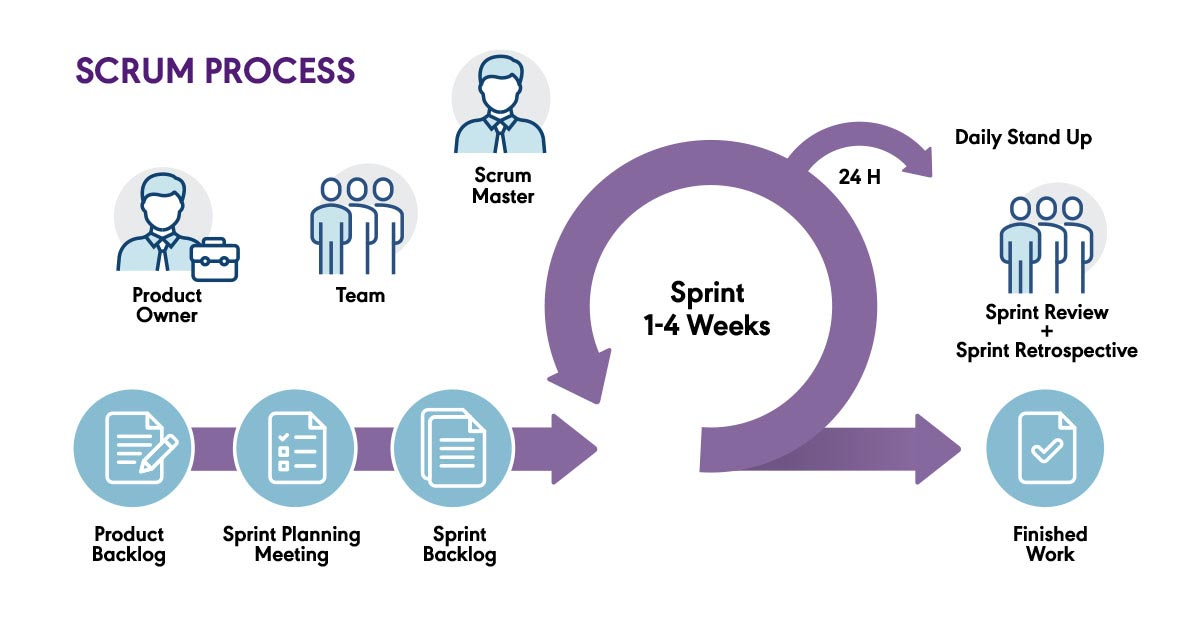
\includegraphics[height=8cm , width=0.8\textwidth]{assets/images/scrum.jpg}
\caption{Methodologie Scrum}
\label{fig:scrum}
\end{figure}

\section{Conclusion}

En conclusion, ce chapitre a mis en lumière la methodologie appliquee dans la conduite du projet de developpement de l'application d'analyse de sentiments pour les commentaires d'Hespress. L'approche methodique de la conception, la rigueur de la planification des taches et l'agilite du developpement ont façonne un outil prometteur pour l'analyse automatisee des opinions publiques.

La maturite du processus adopte reflète notre engagement envers les valeurs d'excellence, de reactivite aux besoins d'analyse et d'innovation constante dans le domaine du traitement automatique du langage naturel.

L'integration entre les technologies de pointe (Next.js, FastAPI, Keycloak, Selenium) et les modeles d'intelligence artificielle avances (XLM-RoBERTa), incarnee par cette application d'analyse de sentiments, est destinee à etablir un nouveau standard en matière d'analyse automatisee des contenus textuels en langue arabe et française.

Avec la fin de ce chapitre, nous anticipons la transition vers les phases subsequentes de mise en œuvre, d'evaluation et d'optimisation, qui seront abordees dans les chapitres suivants. L'impact positif attendu de l'application sur l'analyse des tendances d'opinion et la comprehension des sentiments publics suggère une transformation significative de l'approche d'analyse des donnees textuelles dans le contexte marocain.
